%%%%%%%%%%%%%%%%%%%%%%%%%%%%%%%%%%%%%%%%%%%%%%%%%%%%%%%%%%%%%%%%
%%%%%%%%%%%%%%%%%%%%%%%%%%%%%%%%%%%%%%%%%%%%%%%%%%%%%%%%%%%%%%%%
%%%%
%%%% This text file is part of the source of 
%%%% `Introduction to High-Performance Scientific Computing'
%%%% by Victor Eijkhout, copyright 2012
%%%%
%%%% This book is distributed under a Creative Commons Attribution 3.0
%%%% Unported (CC BY 3.0) license and made possible by funding from
%%%% The Saylor Foundation \url{http://www.saylor.org}.
%%%%
%%%%
%%%%%%%%%%%%%%%%%%%%%%%%%%%%%%%%%%%%%%%%%%%%%%%%%%%%%%%%%%%%%%%%
%%%%%%%%%%%%%%%%%%%%%%%%%%%%%%%%%%%%%%%%%%%%%%%%%%%%%%%%%%%%%%%%

There can be a marked difference between how a parallel algorithm looks to an
observer, and how it is actually programmed.
Consider the case where we have an array of processors~$\{P_i\}_{i=0..p-1}$,
each containing one element of the arrays $x$~and~$y$, and
$P_i$~computes
\begin{equation}
\begin{cases}
y_i\leftarrow y_i+x_{i-1}&i>0\\ \mbox{$y_i$ unchanged}&i=0
\end{cases}
\label{eq:mpi-send-left}
\end{equation}
The global description of this could be
\begin{itemize}
\item Every processor $P_i$ except the last sends its $x$ element to~$P_{i+1}$;
\item every processor $P_i$ except the first receive an $x$ element from
  their neighbour~$P_{i-1}$, and
\item they add it to their $y$ element.
\end{itemize}
However, in general we can not code in these global terms.
In the \ac{SPMD} model (section~\ref{sec:spmd}) each
processor executes the same code, and the overall algorithm
is the result of  these individual behaviours. 
The local program has access only to local data --~everything else
needs to be communicated with send and receive operations~-- and the
processor knows its own number.

One possible way of writing this would be
\begin{itemize}
\item If I am processor~0 do nothing, otherwise receive a $y$ element
  from the left, add it to my $x$ element.
\item If I am the last processor do nothing, otherwise send my $y$
  element to the right.
\end{itemize}
At first we look at the case where sends and
receives are so-called \indexterm{blocking communication}
instructions: a send instruction does not finish until the sent item
is actually received, and a receive instruction waits for the
corresponding send. This means that sends and receives between
processors have to be carefully paired. We will now see that this can
lead to various problems on the way to an efficient code.

The above solution is illustrated in figure~\ref{fig:wave_right_1},
where we show
\begin{figure}
  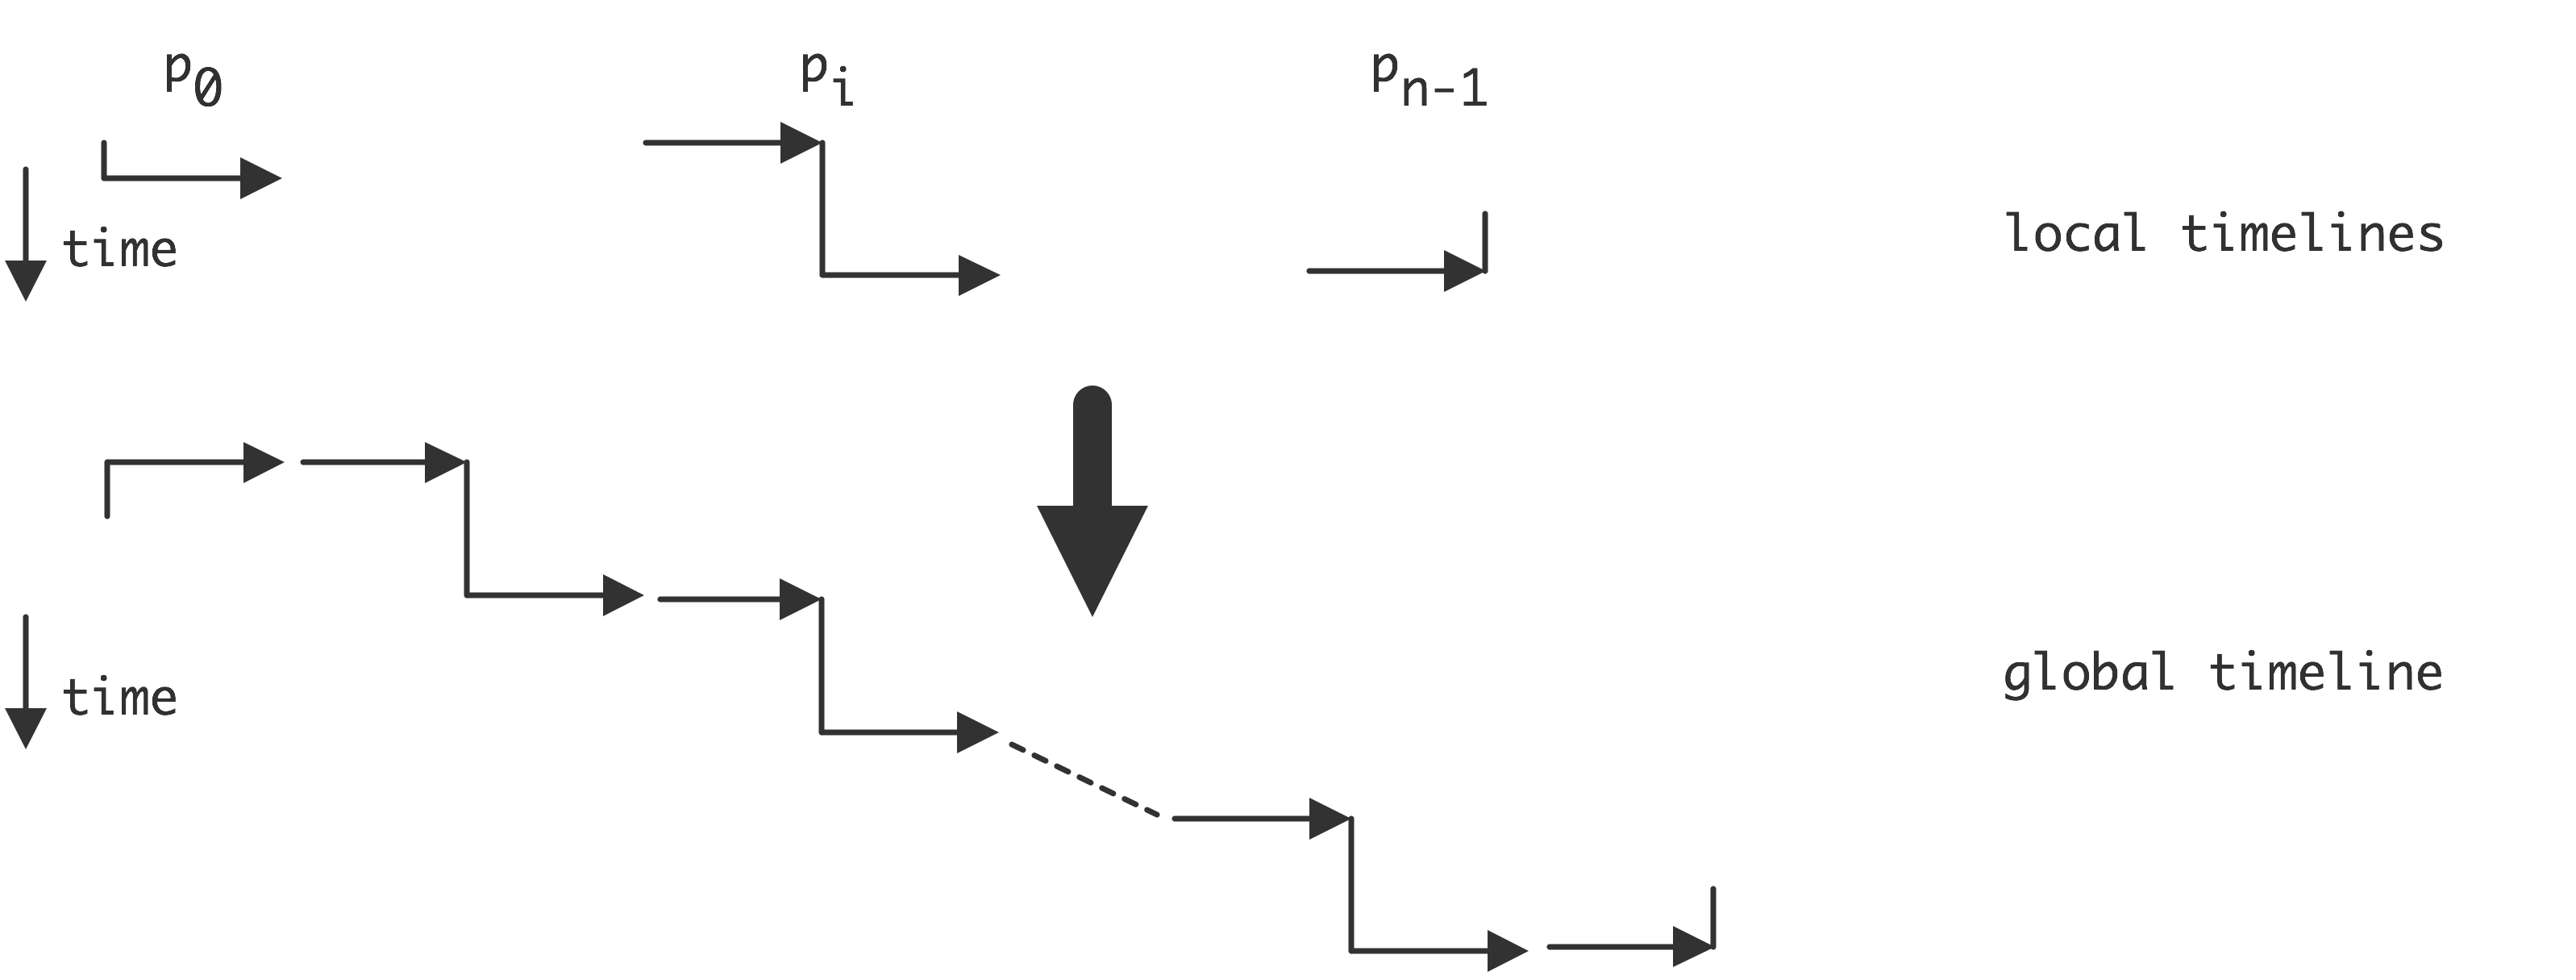
\includegraphics[scale=.14]{graphics-public/wave_right_1}
  \caption{Local and resulting global view of an algorithm for sending
    data to the right}
  \label{fig:wave_right_1}
\end{figure}
the local timelines depicting the local processor code, and the resulting
global behaviour. You see that the processors are not working at the
same time: we get \indexterm{serialized execution}.

What if we reverse the send and receive operations?
\begin{itemize}
\item If I am not the last processor, send my $x$ element to the
  right;
\item If I am not the first processor, receive an $x$ element from the
  left and add it to my $y$ element.
\end{itemize}
This is illustrated in figure~\ref{fig:wave_right_2} and you see that
\begin{figure}
  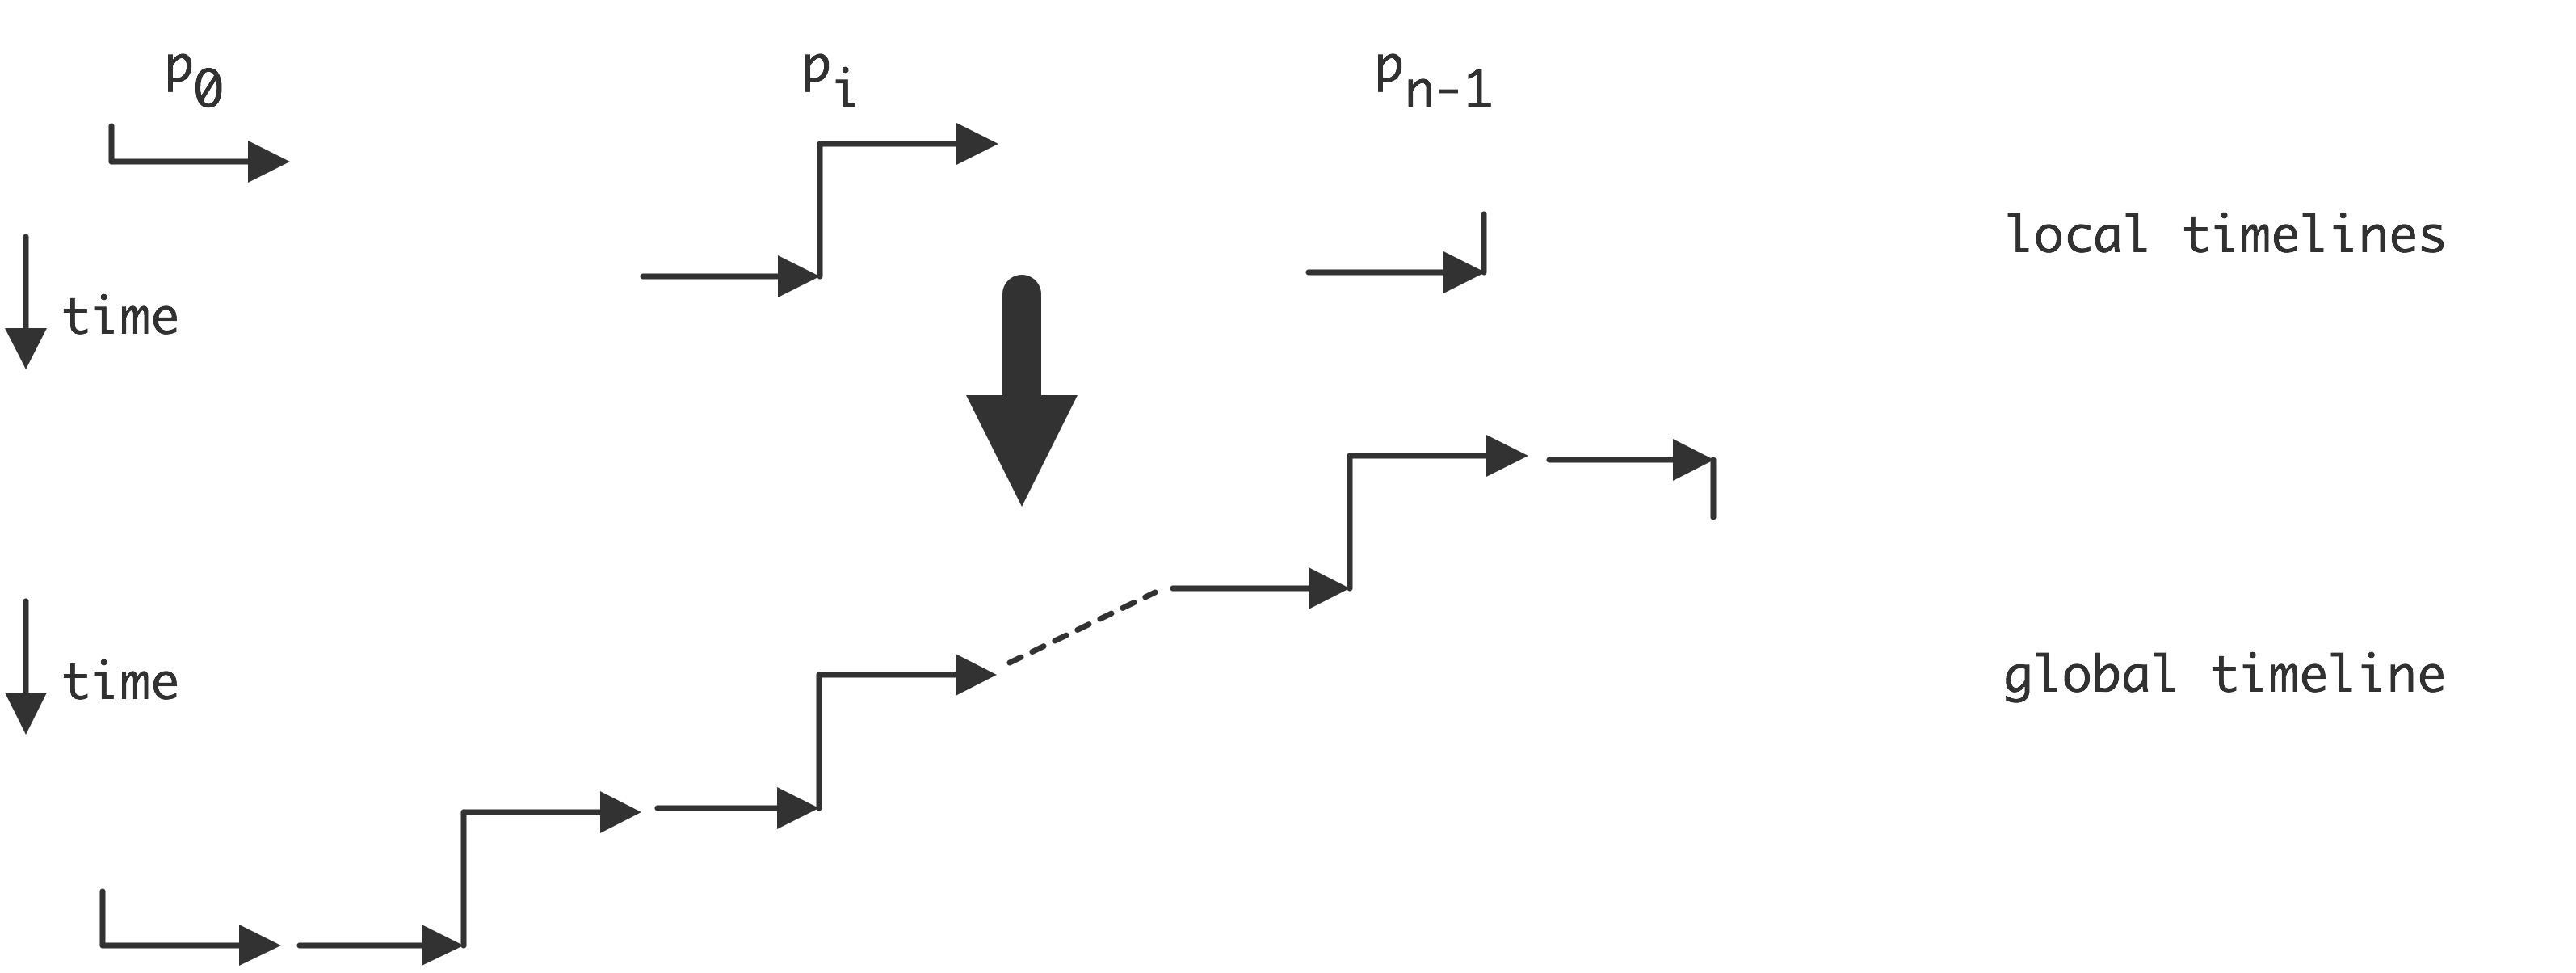
\includegraphics[scale=.14]{graphics-public/wave_right_2}
  \caption{Local and resulting global view of an algorithm for sending
    data to the right}
  \label{fig:wave_right_2}
\end{figure}
again we get a serialized execution, except that now the processor are
activated right to left.

If the algorithm in equation~\ref{eq:mpi-send-left} had been cyclic:
\begin{equation}
\begin{cases}
y_i\leftarrow y_i+x_{i-1}&i=1\ldots n-1\\ 
y_0\leftarrow y_0+x_{n-1}&i=0
\end{cases}
\label{eq:cyclic-add}
\end{equation}
the problem would be even worse. Now the last processor can not start
its receive since it is blocked sending~$x_{n-1}$ to processor~0. This
situation, where the program can not progress because every processor is
waiting for another, is called \indexterm{deadlock}. 

The solution to getting an efficient code is to make as much of the
communication happen simultaneously as possible. After all, there are
no serial dependencies in the algorithm. Thus we program the algorithm
as follows:
\begin{itemize}
\item If I am an odd numbered processor, I send first, then recieve;
\item If I am an even numbered processor, I receive first, then send.
\end{itemize}
This is illustrated in figure~\ref{fig:wave_right_3}, and we see that
\begin{figure}
  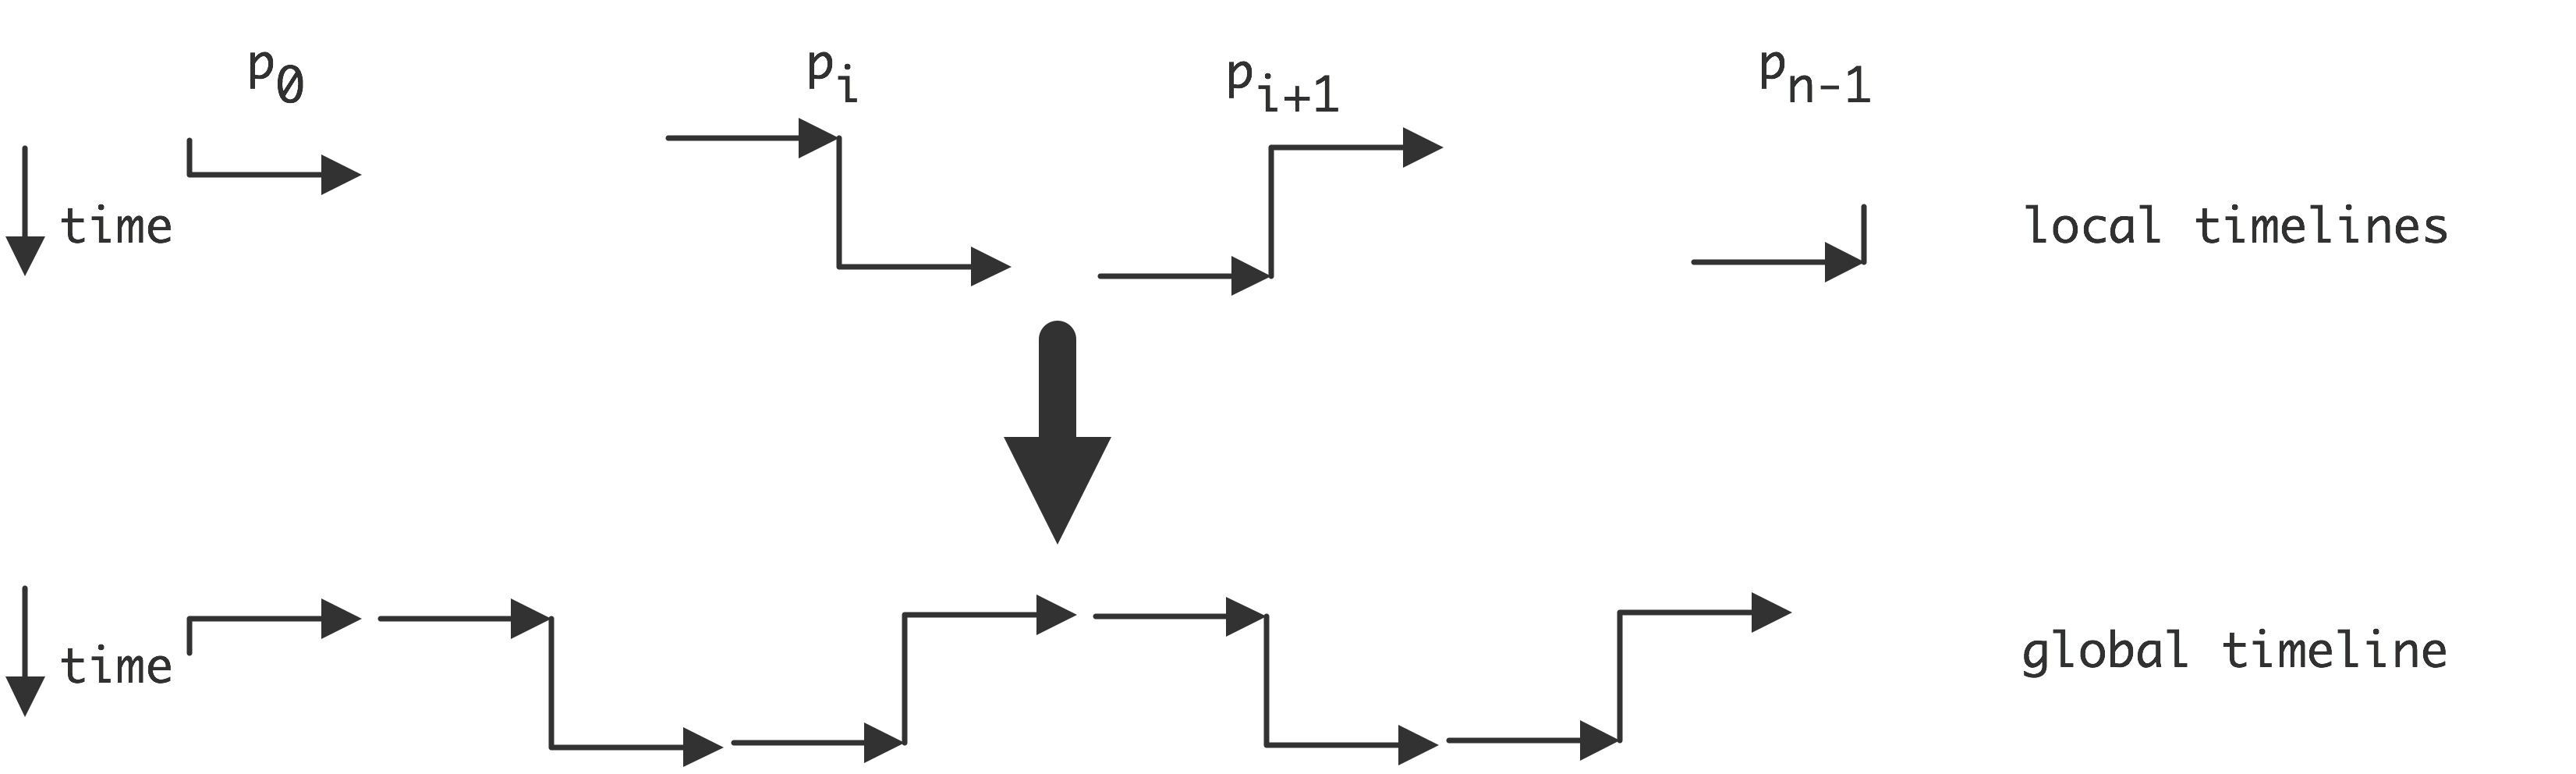
\includegraphics[scale=.115]{graphics-public/wave_right_3}
  \caption{Local and resulting global view of an algorithm for sending
    data to the right}
  \label{fig:wave_right_3}
\end{figure}
the execution is now parallel.

\Level 2 {Blocking and non-blocking communication}

The reason for blocking instructions is to prevent accumulation of
data in the network. If a send instruction were to complete before the
corresponding receive started, the network would have to store the
data somewhere in the mean time.
Consider a simple example:
\begin{verbatim}
buffer = ... ;  // generate some data
send(buffer,0); // send to processor 0
buffer = ... ;  // generate more data
send(buffer,1); // send to processor 1
\end{verbatim}
After the first send, we start overwriting the buffer. If the data in
it hasn't been received, the first set of values would have to be
buffered somewhere in the network, which is not realistic.
By having the send operation block,
the data stays in the sender's buffer until it is guaranteed to have
been copied to the recipient's buffer.

One way out of the problem of sequentialization or deadlock that
arises from blocking instruction is the use
of \indexterm{non-blocking communication} instructions, which include
explicit buffers for the data. With non-blocking send instruction, the
user needs to allocate a buffer for each send, and check when it is
safe to overwrite the buffer.
\begin{verbatim}
buffer0 = ... ;   // data for processor 0
send(buffer0,0);  // send to processor 0
buffer1 = ... ;   // data for processor 1
send(buffer1,1);  // send to processor 1
...
// wait for completion of all send operations.
\end{verbatim}

